\documentclass[../report.tex]{subfiles}
\graphicspath{{\subfix{../image/}}}

\begin{document}
\subsection{Research and Evaluation for Loadcell-Interfacing}
A Load Cell serves as a sensor that transforms applied force, encompassing pressure, rotational force, compression,
or tension, into quantifiable electrical signals.

\subsubsection{Choice of loadcells}

One of the functionalities of the forklift is measuring the weight lifted.
This serves the purpose of ensuring safe operations not only for customers, 
but also preventing the forklift from tilting or damaging itself in one way or the other.

In addition load cells inside the fork allow for a low level pallet detection, enabling 
the forklift to drop off pallets at any height, for example on top of another pallet of undefined 
dimensions. 

In accordance to the set requirements, the forklift should at least lift 3.5kg.
Hence, the loadcells should be able to withstand this weight. 
Next to buying new loadcells, one possible option is to take the loadcells
out of a kitchen scale rated for that weight. This is beneficial in serveral aspects.
Not only does it give a insight into reverse engineering, but also provides beneficial
insight in classifying unknown sensor characteristics. Furthermore, it does not 
stress the budget. 

\begin{figure}[H]
  \centering
  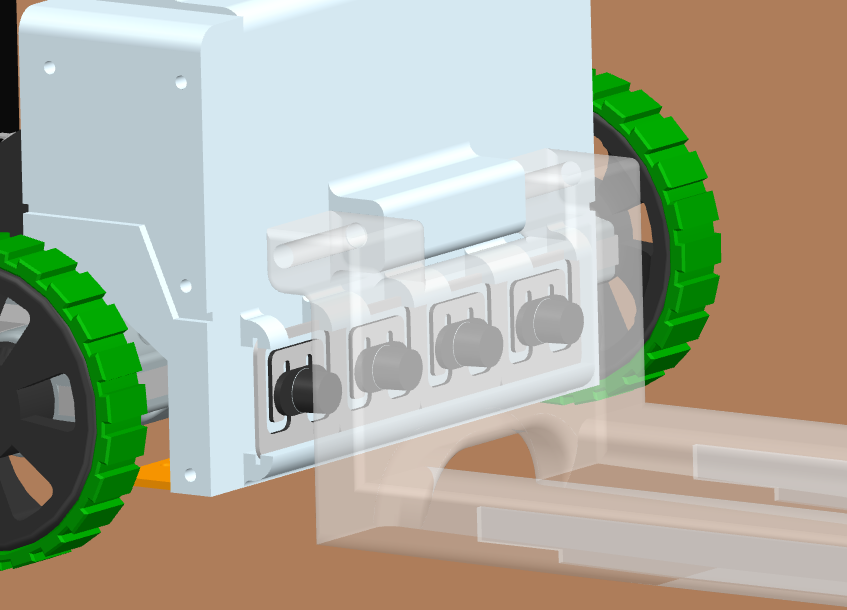
\includegraphics[width=0.7\textwidth]{loadcellarray.png}
  \caption{Assembly configuration of Loadcells}
\end{figure}

A kitchen scale rated for max. 5kg was bought. The four loadcells of this scale were taken to the lab and
their behavior was evaluated. 

Conclusion: The loadcells suit the application. They can not only withstand the
required stress-requirements, but also work reliable. Moreover, they fulfill the 
space requirements for the "small-scale" fork. Furthermore, they bring a considerable
learning effect with them.

The next engineering challenge is interfacing these loadcells.
These loadcells include two variable resistances, a strain gauge. One of them increases
with stress the other one decreases with stress. 

Interfacing bears several challenges:

\begin{itemize}

  \item Output of interface must be compatible with ADC range of microcontroller.
  \item Current through loadcells must be limited.
  \item Output needs to be amplified.

\end{itemize}
\begin{figure}[H]
  \centering
  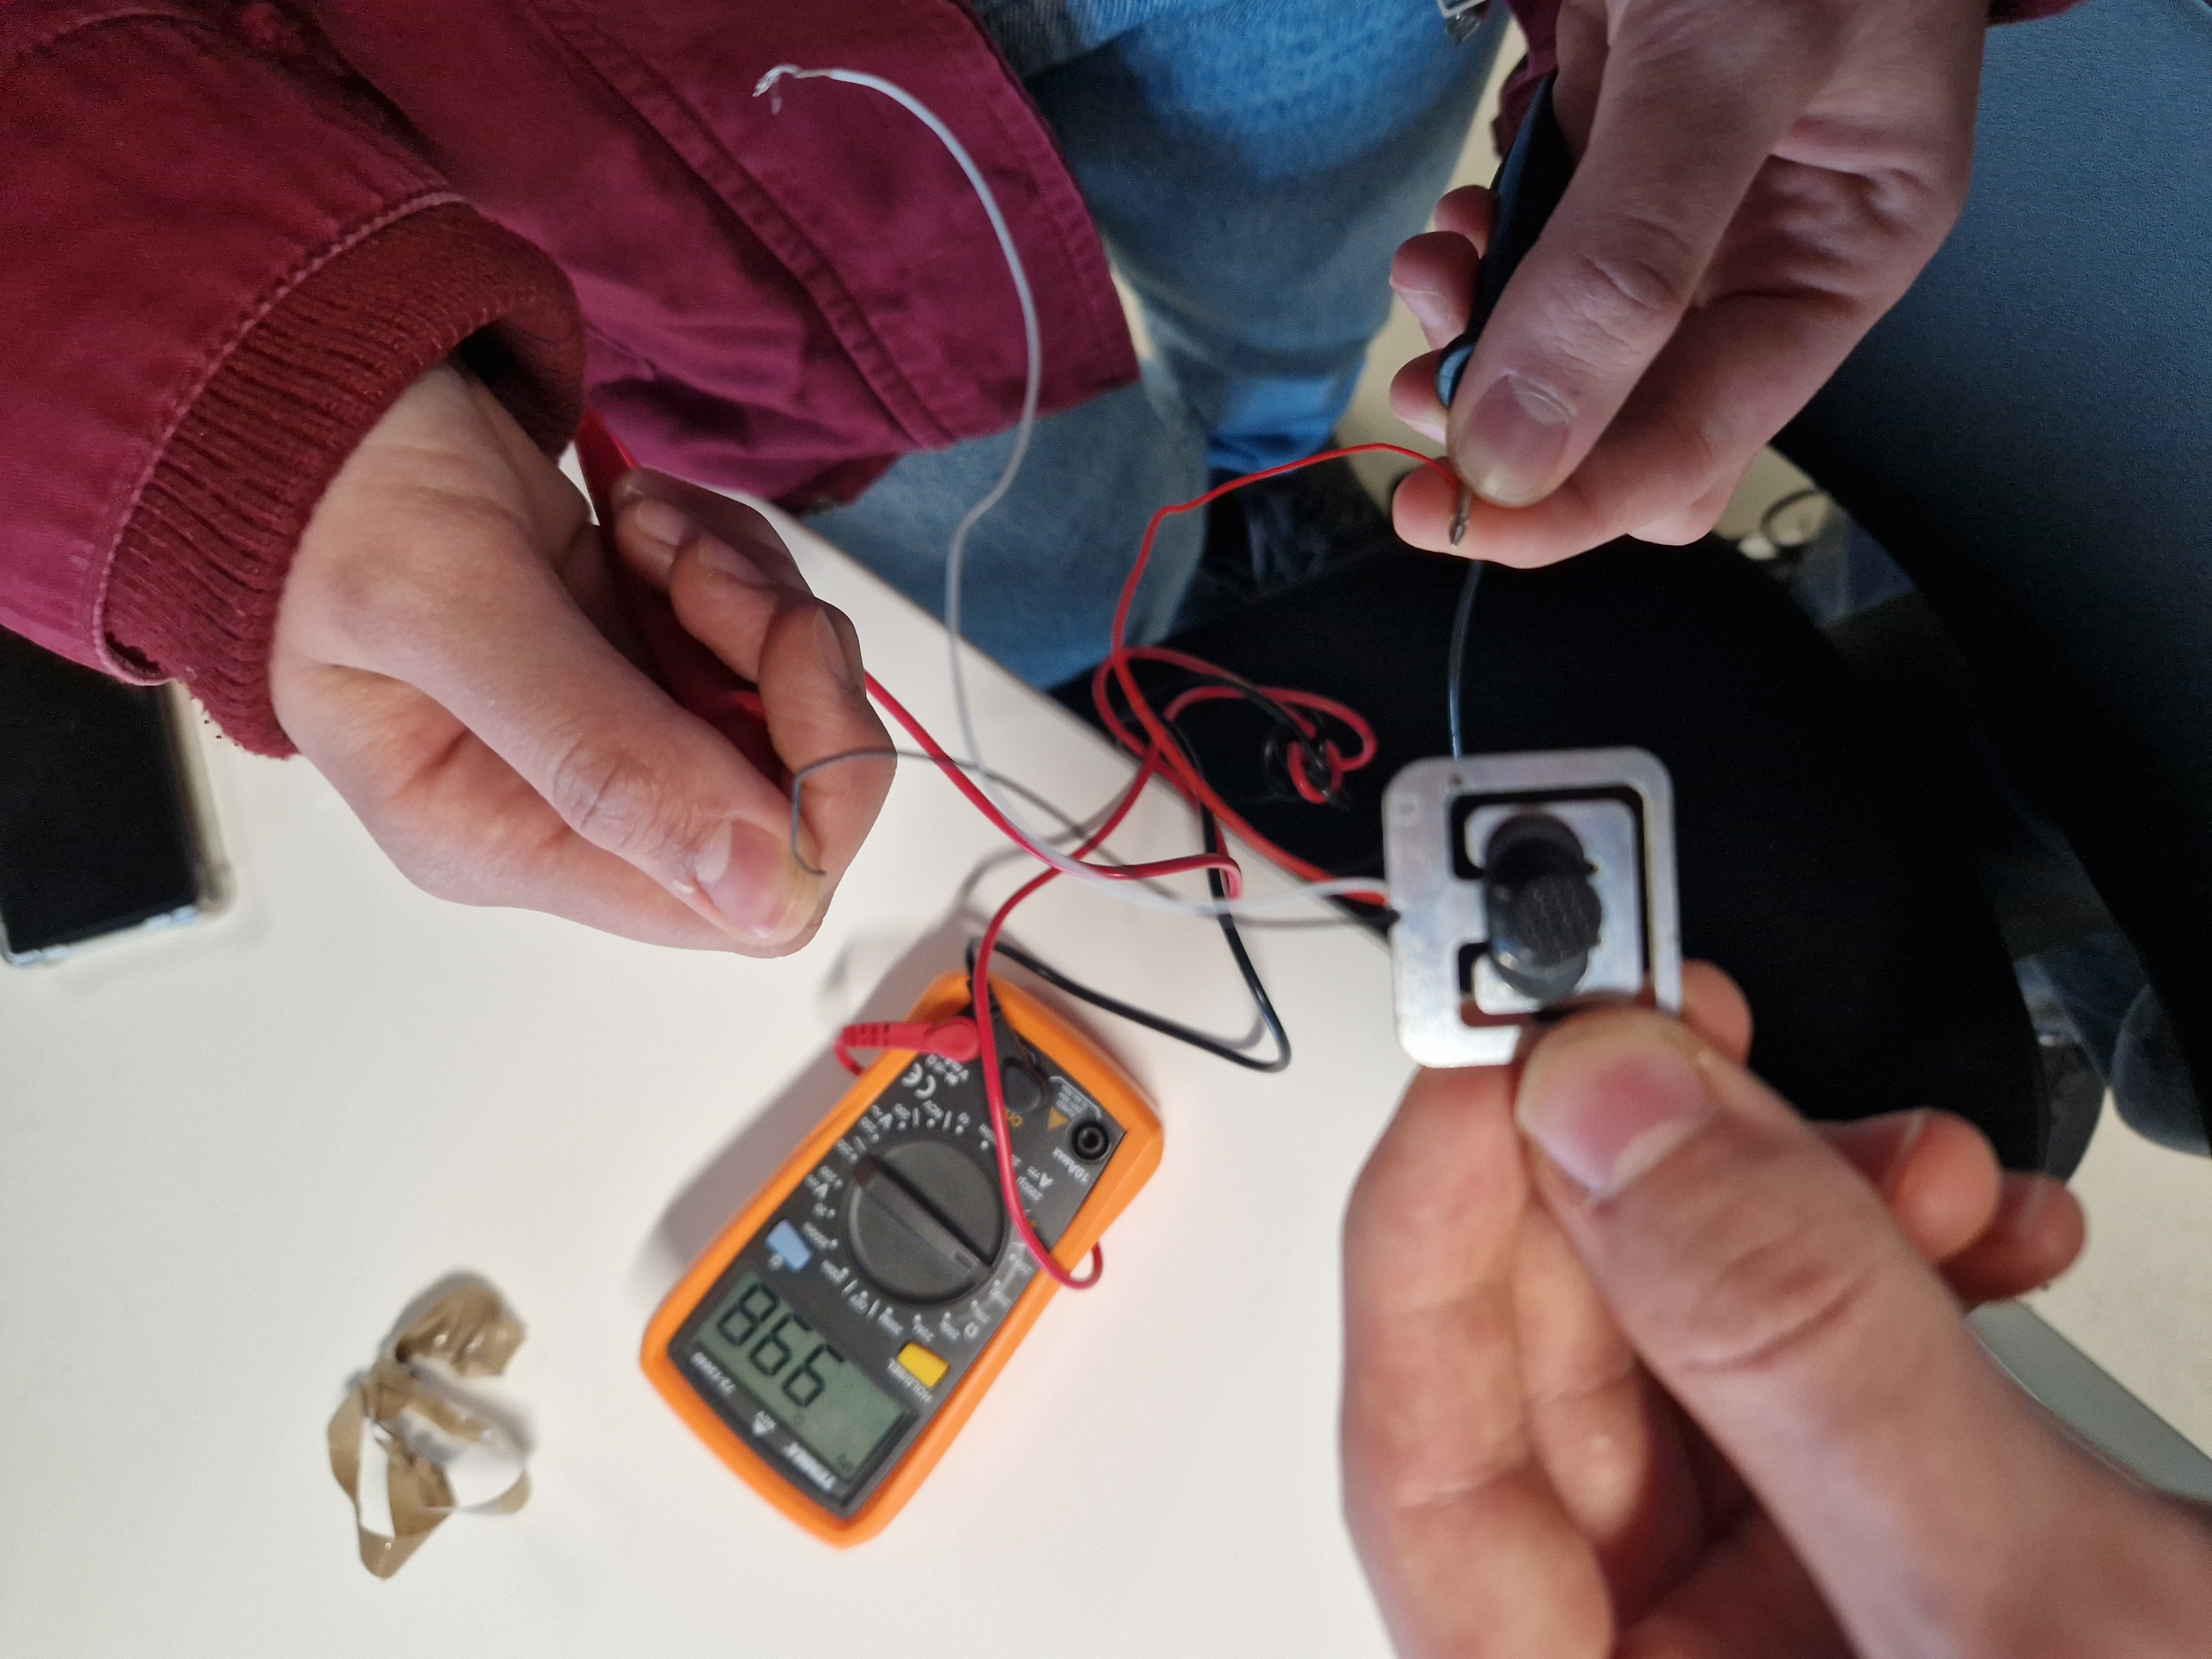
\includegraphics[width=0.75\linewidth]{loadcell_testing.jpg}
  \caption{Testing the loadcells}
\end{figure} 
\subsubsection{Available Interface Options}

In this section the available options to overcome these challenges are discussed.

\begin{itemize}
  
  \item HX711 Interface Module and load-cell
  \item Wheatstone bridge - in different configurations
  \begin{itemize}
    \item With constant current source
    \item Without constant current source
  \end{itemize}
  
\end{itemize}

\subsubsection{HX711 Interface Module and load-cell}

The load cell generates an output in changing resistance; therefore, it is essential to magnify 
this signal into a higher-level amplitude and subsequently convert it into a digital format for further processing.
To accomplish this task, the HX711 interface module could be used. This was recommended by a professor. 
This module serves to amplify the load cell's output into voltage and transmit it to the microcontroller for weight calculation. 
The illustration below depicts the HX711 interface module.


\begin{figure}[H]
  \centering
  \begin{subfigure}[b]{0.4\linewidth}
    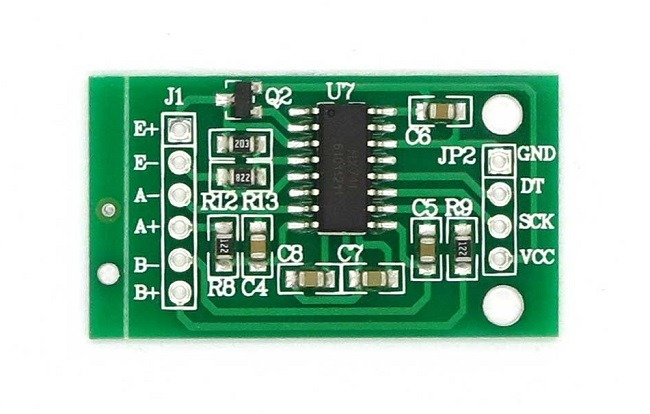
\includegraphics[width=\linewidth]{image/HX711-Weighing-Sensor-Dual-Channel-24-Bit-Precision-A-D-Module-Pressure-Sensor_1.jpg}
    \caption{HX711 Interface Module }
  \end{subfigure}
  \begin{subfigure}[b]{0.4\linewidth}
    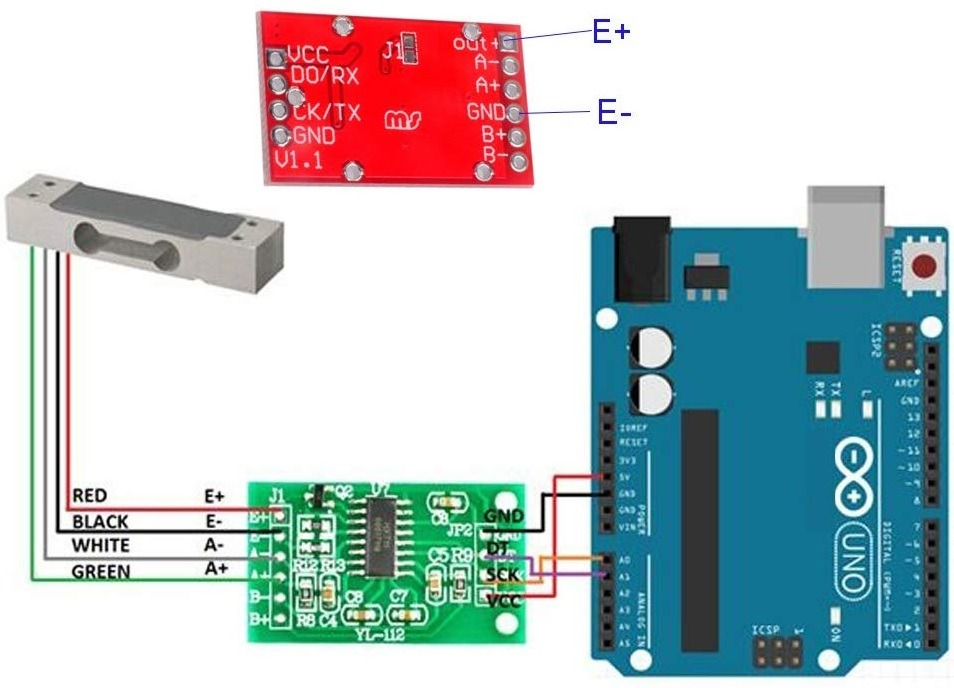
\includegraphics[width=\linewidth]{image/hx711-red.jpg}
    \caption{HX711 Interface Module and Load cell using Arduino}
  \end{subfigure}
  
  
\end{figure}

\subsubsection{Wheatstone bridge - in different configurations}

Another option for getting valuable data about the weight from the loadcells
is to make a wheatstone bridge and build a self-designed amplifying circuit.
This would come with significant learning progress in the sense of the task and 
focus this semester.

\begin{figure}[H]
  \centering
  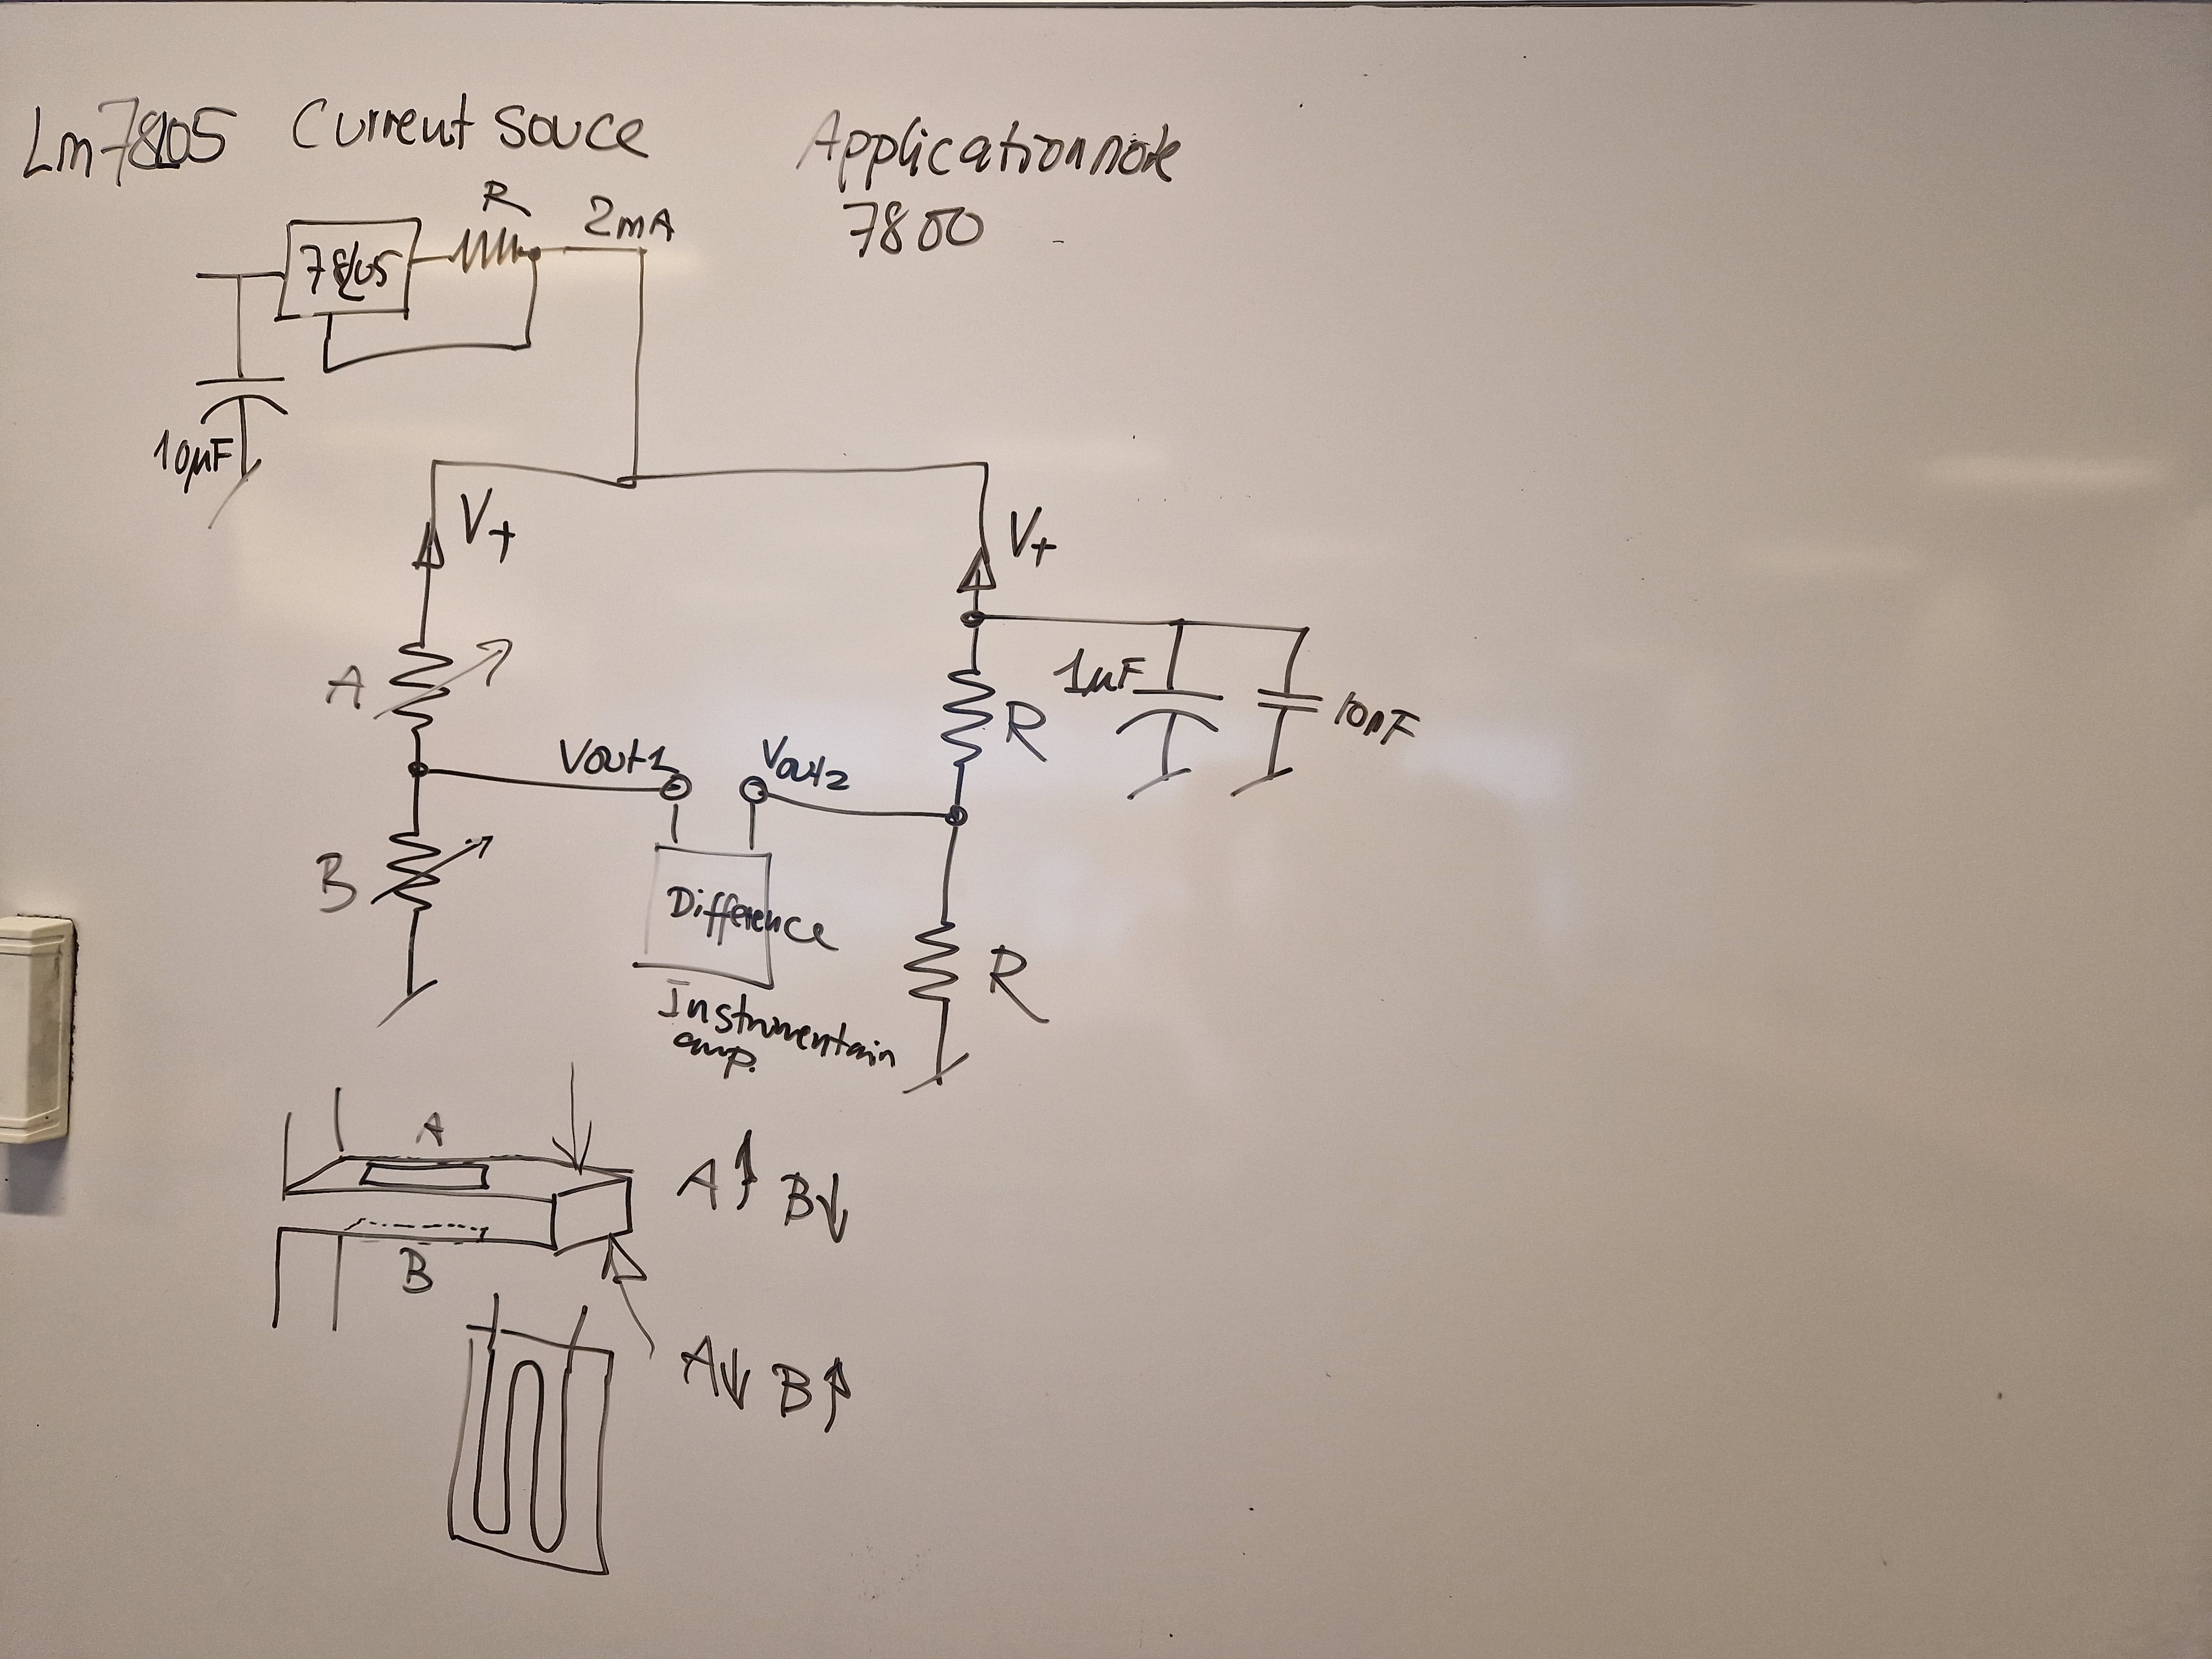
\includegraphics[width=0.75\linewidth]{loadcell_interface_ci.jpg}
  \caption{Potential setup using one loadcell and constant current source}
\end{figure} 

\subsubsection{The decision}
It was decided to go with the wheatstone-bridge option - the main reason being
the fundamental learning experience. Using a premade module would not give much 
learning experience with analog sensors in the end. 

\quad
Thus, after the first step of the engineering method - evaluation of options -
designs were made an tested.
It also was decided to omit the constant current source, as this would have been an 
overcomplicated setup. The calculations done showed that with a voltage source of 3.3V
the current through the loadcells would be in the range of a few mA. This was also backed
by simulations of equivalent voltage dividers in LTSpice.
The following picture shows a first working prototype - back then the setup included just one loadcell. 
\begin{figure}[H]
  \centering
  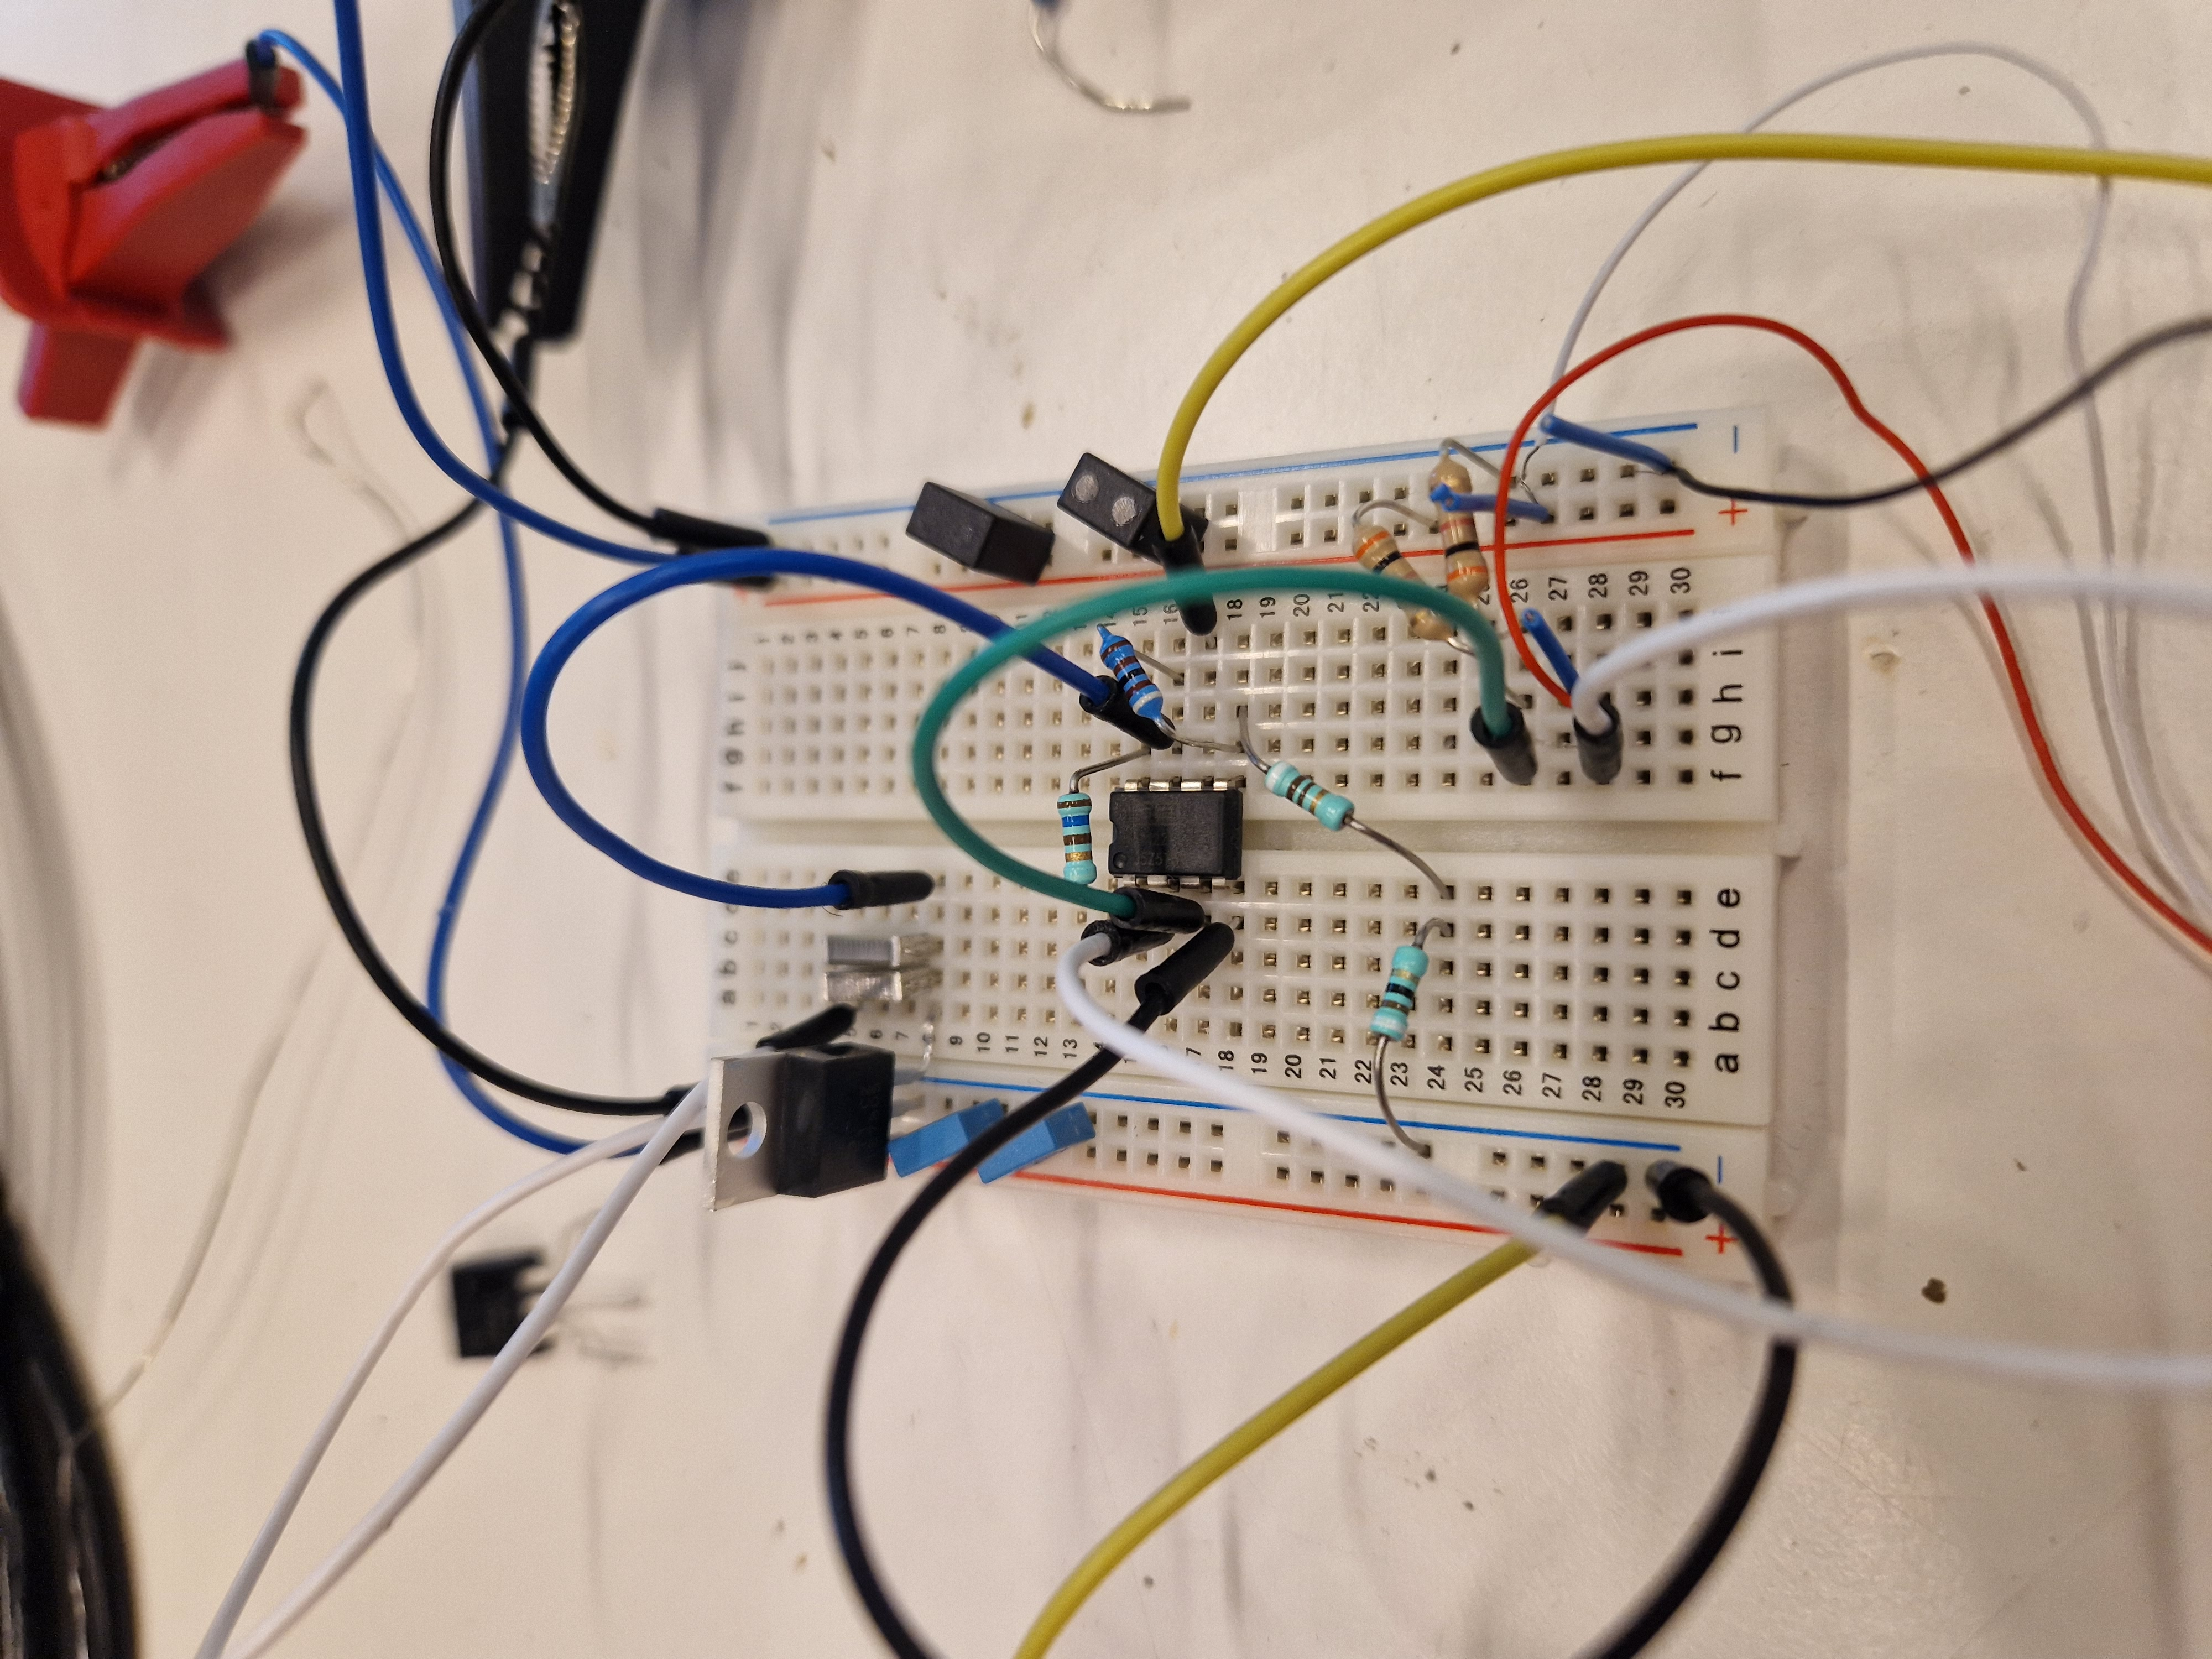
\includegraphics[width=0.5\textwidth]{first_prototype_loadcell.jpg}
  \caption{First working prototype of the loadcell amplifier}
\end{figure}

Nonetheless, the setup got improved 
and extended to the final implementation:
\subsubsection{Wheatstone bridge - The final implementation}

The loadcells are made of a bending material and strain gauges, which are resistive
sensors that increase their resistance when tensioned and decrease when compressed.
In the final design we went with using all 4 load cells in the wheatstone-bridge formation
where 2 will get tensioned, 2 compressed and then wired inverted to create the biggest change
in ratio once pressed. Or effectively creating two voltage dividers with one rising the voltage
and the other one decreasing starting at the same point.

From there we already got two stable output voltages with difference in the millivolt range, 
which than had to be amplified.
As the Ws-Bridge gives out two voltages we used the INA122p instrumentation amplifier and 
configured it with a gain of 308 to have our maximum output voltage under full load just 
under 2.5V which is the maximum adc input voltage for the ESP32.

\begin{figure}[H]
  \centering
  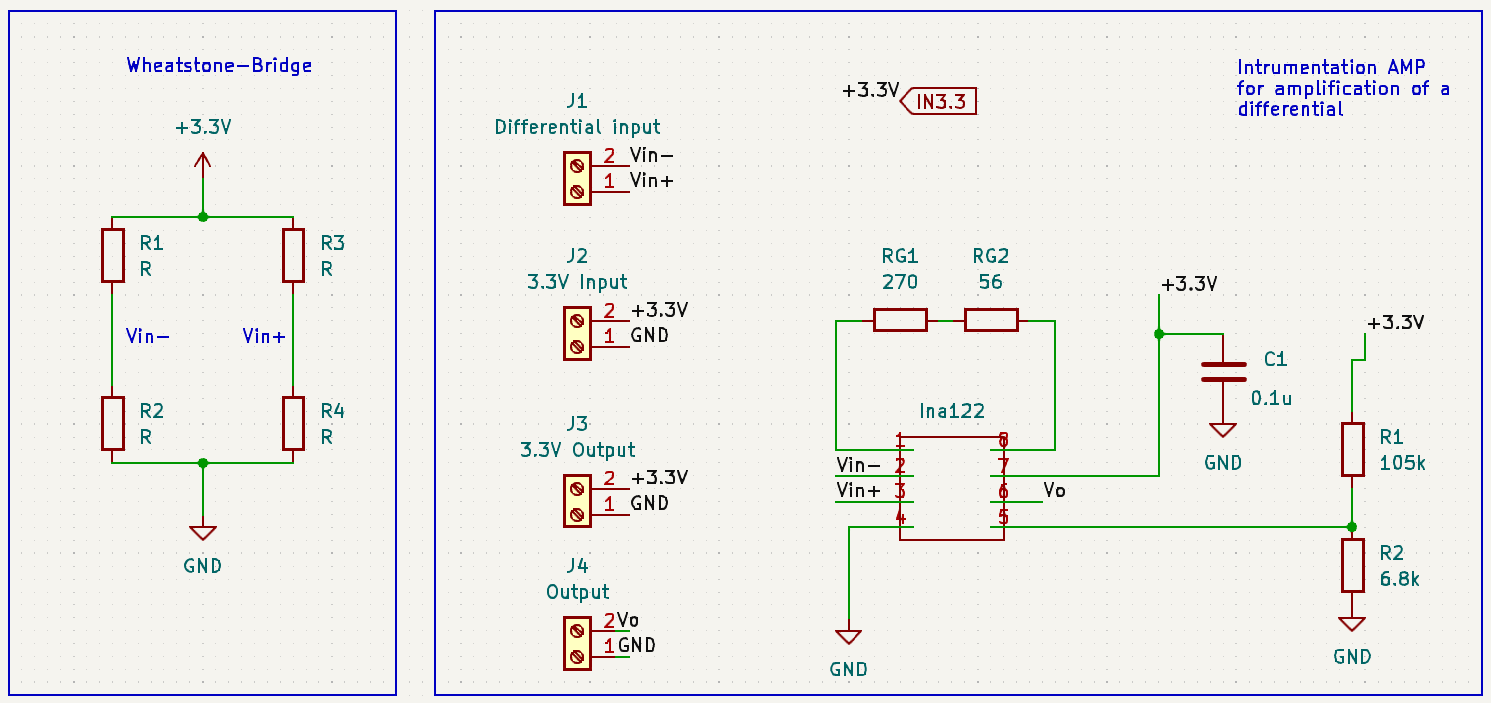
\includegraphics[width=0.85\linewidth]{ampcircuit.png}
  \caption{LoadCell Schematics}
\end{figure} 
\begin{figure}[H]
  \centering
  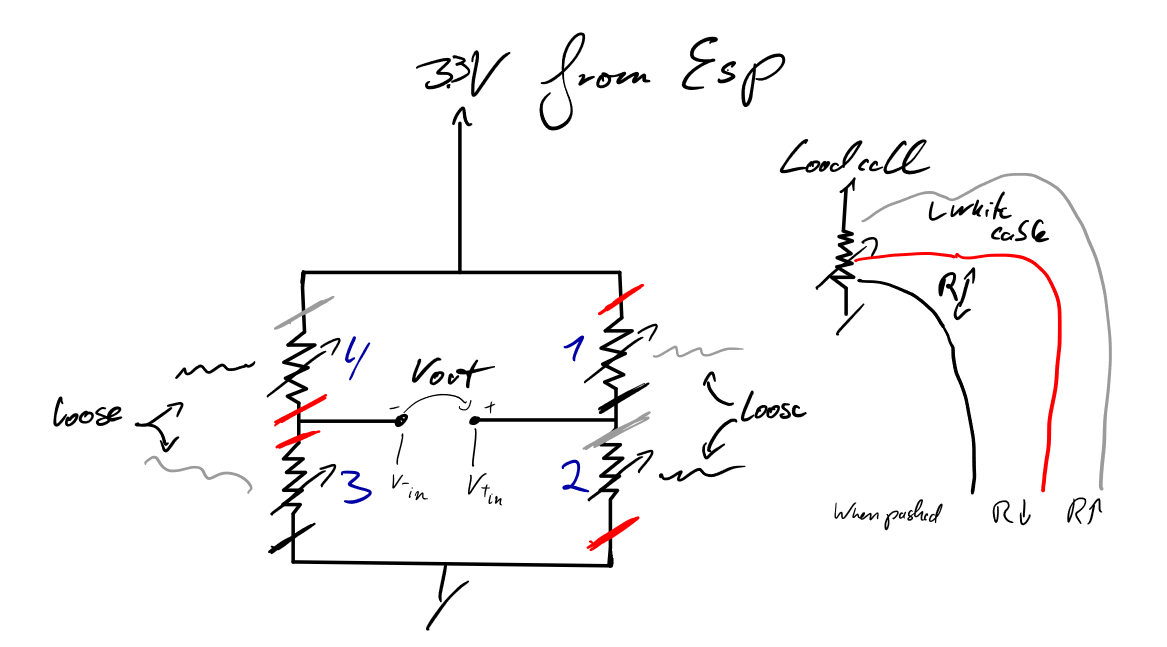
\includegraphics[width=0.5\textwidth]{Ws-Bridge-wiring.png}
  \caption{Wiring for achieving maximum potential difference}
\end{figure}

The Ws-Bridge was then directly mounted onto the Mast-Assembly, while the amplifier circuit 
was manufactured as a PCB and mounted on the base body.

\begin{figure}[H]
  \centering
  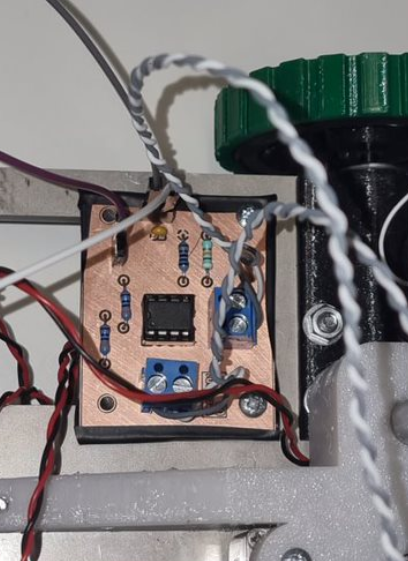
\includegraphics[width=0.44\linewidth]{ampPCB.png}
  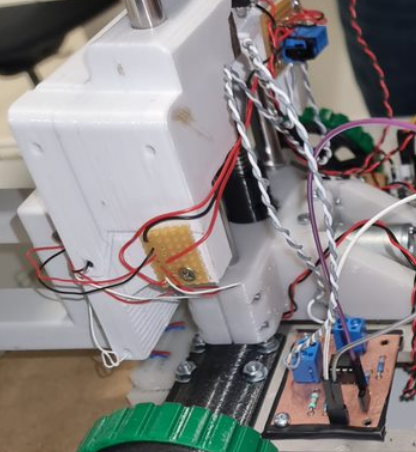
\includegraphics[width=0.55\linewidth]{Ws-Bridge.png}
  \caption{AmpPCB and Ws-Bridge}
\end{figure} 

\subsubsection{Calibrating the output and slight adjustments}
Of course the measured analog voltage has to be converted to a weight.
Through testing it has been determined that the output can be approximated
by an ideal-straight line. The sensitivity has then be determined by putting no load
and 500g (centered) on the fork. Then the corresponding conversion functions have been 
implemented in code - see coding section.
While calibrating it was also noticed that the initial gain of the op amp is too strong as it 
surpasses the ESP32´s ADC range.
The weight of the fork itself biases the wheatstone bridge. This is, of course, also amplified.
Thus, the gain resistor was adjusted slightly to decrease the gain.

\quad
When placing a 500g weight the converted result will oscillate between about 450g and 550g.
This issue could be tackled by implementation of a digital filter - averaging. Prints of these testings
can be found in the code repository.
\quad

The implementation did not just bring the team out of the comfort zone of premade modules, but
also led to applying knowledge from the course Sensors and Actuators.

\end{document}